%%%
%%% Now we have to get the source code in as a set of Appendices.
%%% Source code will be Appendix A, with each file numbered X.y
%%%
\appendix
%
%%%
%%% -> \chapter will cause the next bit to be labelled Appendix A
%%% -> \section will give us A.1, \subsection A.1.1 etc.
%%%
%%% I suggest a section for each program and a subsection for each file
%%% in the program.  Alternatively, a chapter for each program, a
%%% section for each library and a subsection for each file.
%%%
%
\linespread{1}
\chapter{Papers associated with this thesis}
\section{Preface}
The following paper is a summary of a \textit{Legionella mcdadei} genome assembly project that I worked on with collaborators at the University of Canterbury and the University of Otago. \textit{ Legionella mcdadei} is a bacterial pathogen that can cause a severe form of pneumonia called Legionnaire's disease, which is especially prevalent in New Zealand. The genomes of two isolates of \textit{L. mcdadei} from New Zealand patients presenting with Legionnaire's disease were sequenced, assembled and annotated.

This paper is published as follows:
Osborne AJ, \textbf{Jose BR}, Perry J, Smeele Z, Aitken J, Gardner PP, Slow S. 2017. Complete genome sequences of two geographically distinct \textit{Legionella micdadei} clinical isolates. \textit{Genome Announc} 5:e00436-17. DOI: 10.1128/genomeA.00436-17

\section{Contributions}
I performed the genome assembly, annotation and comparison, submitted the data to NCBI and worked on the methods for the draft of the paper. 
\newpage
\begin{figure}
    \centering
    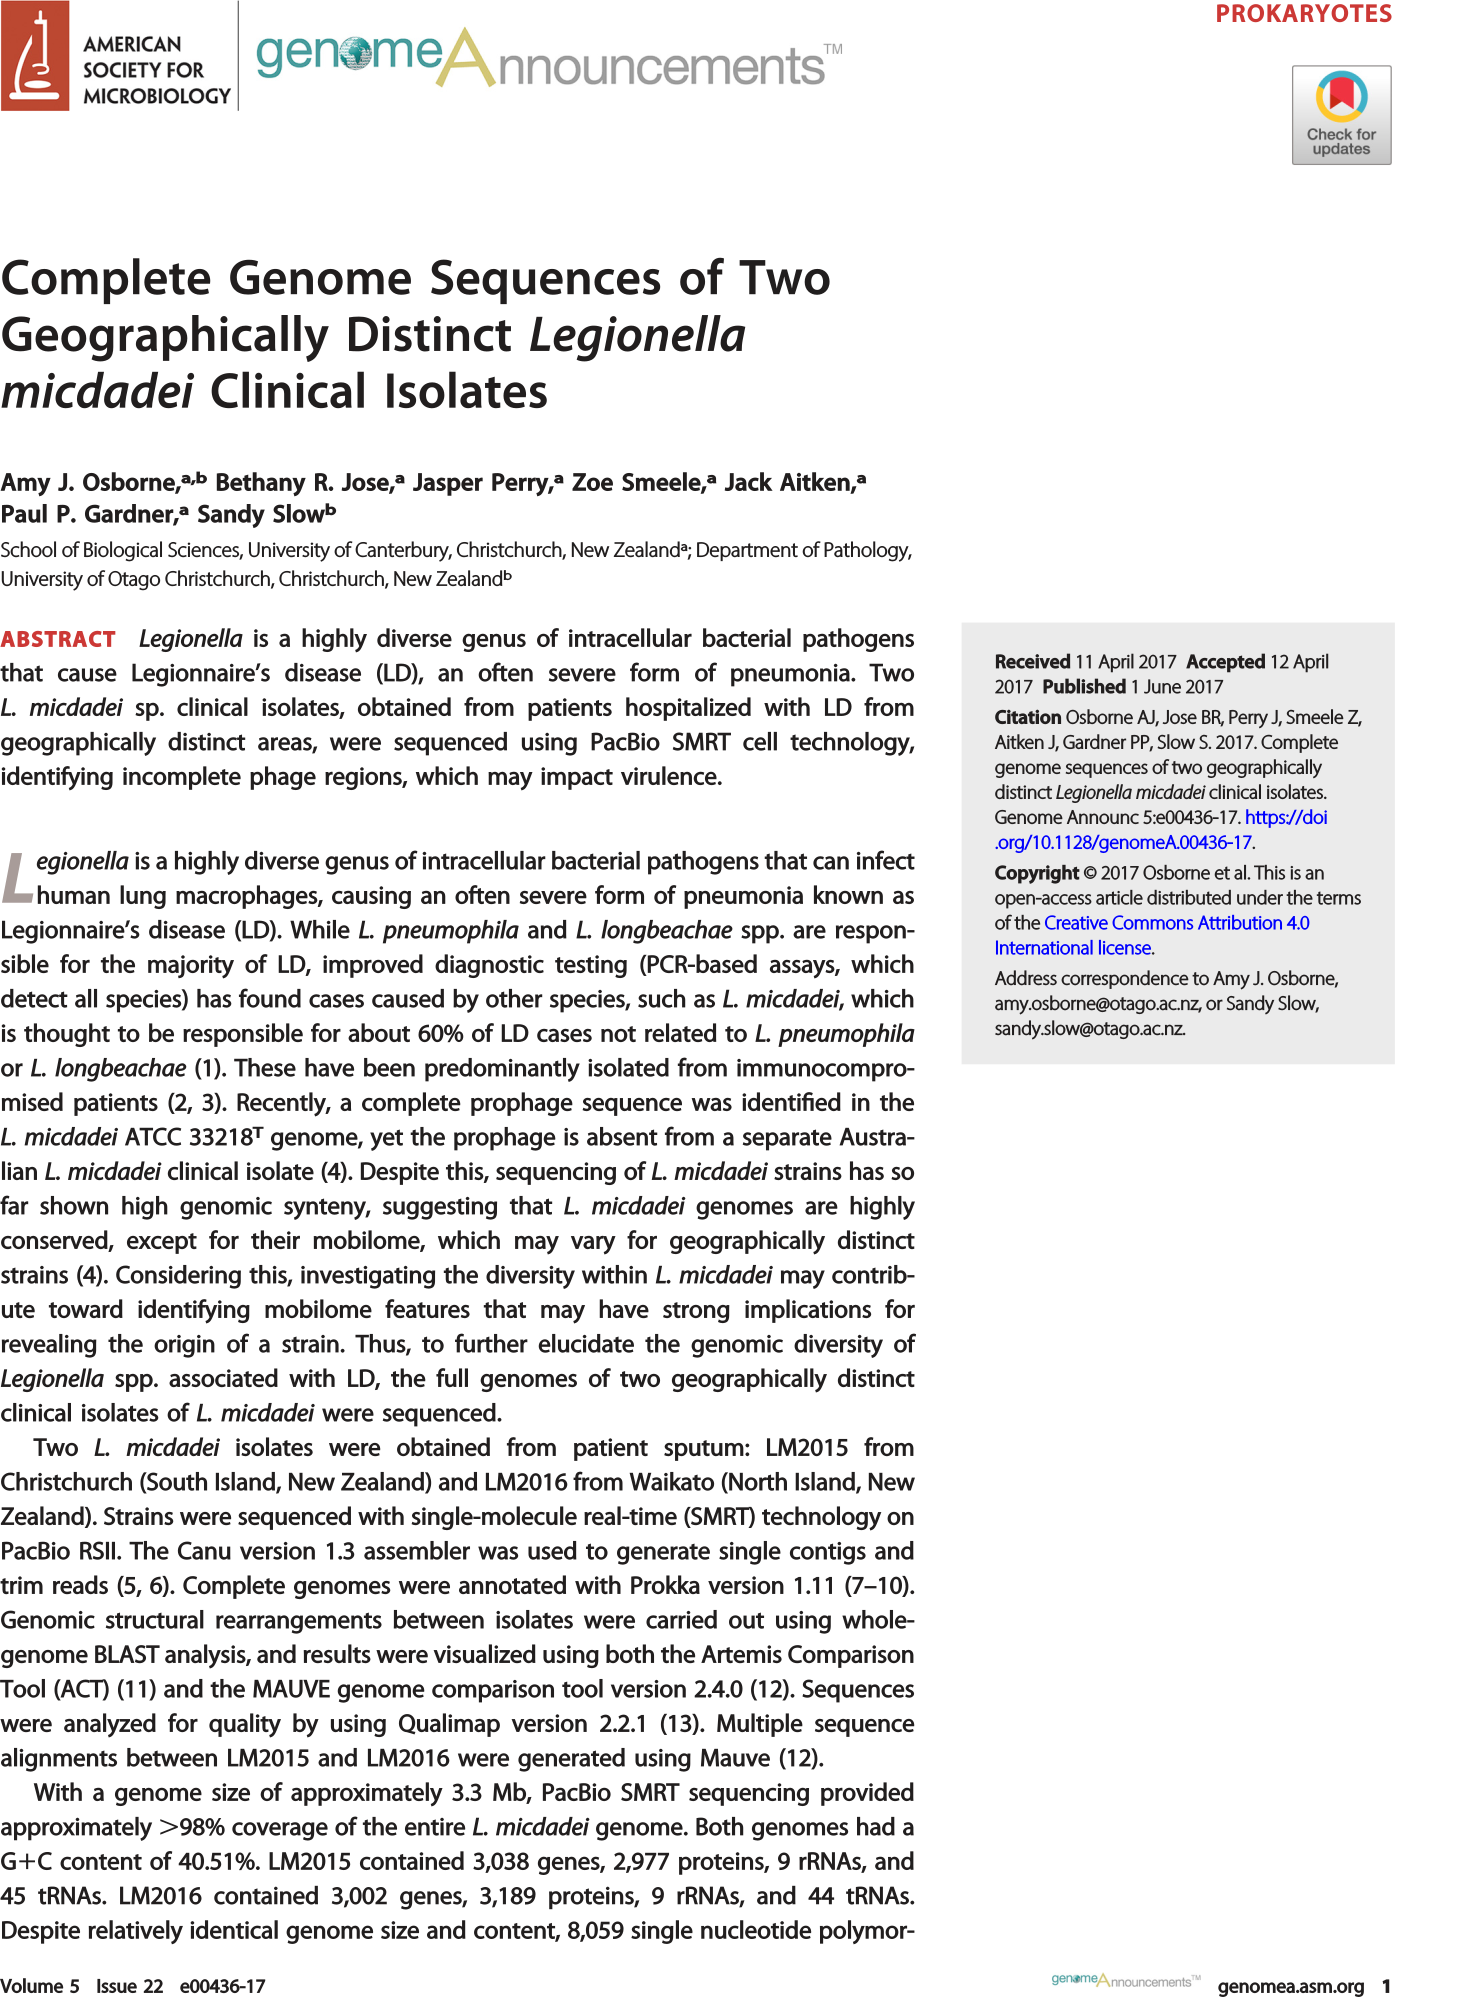
\includegraphics[width=\linewidth]{other/legionella_1.png}
\end{figure}
\begin{figure}
    \centering
    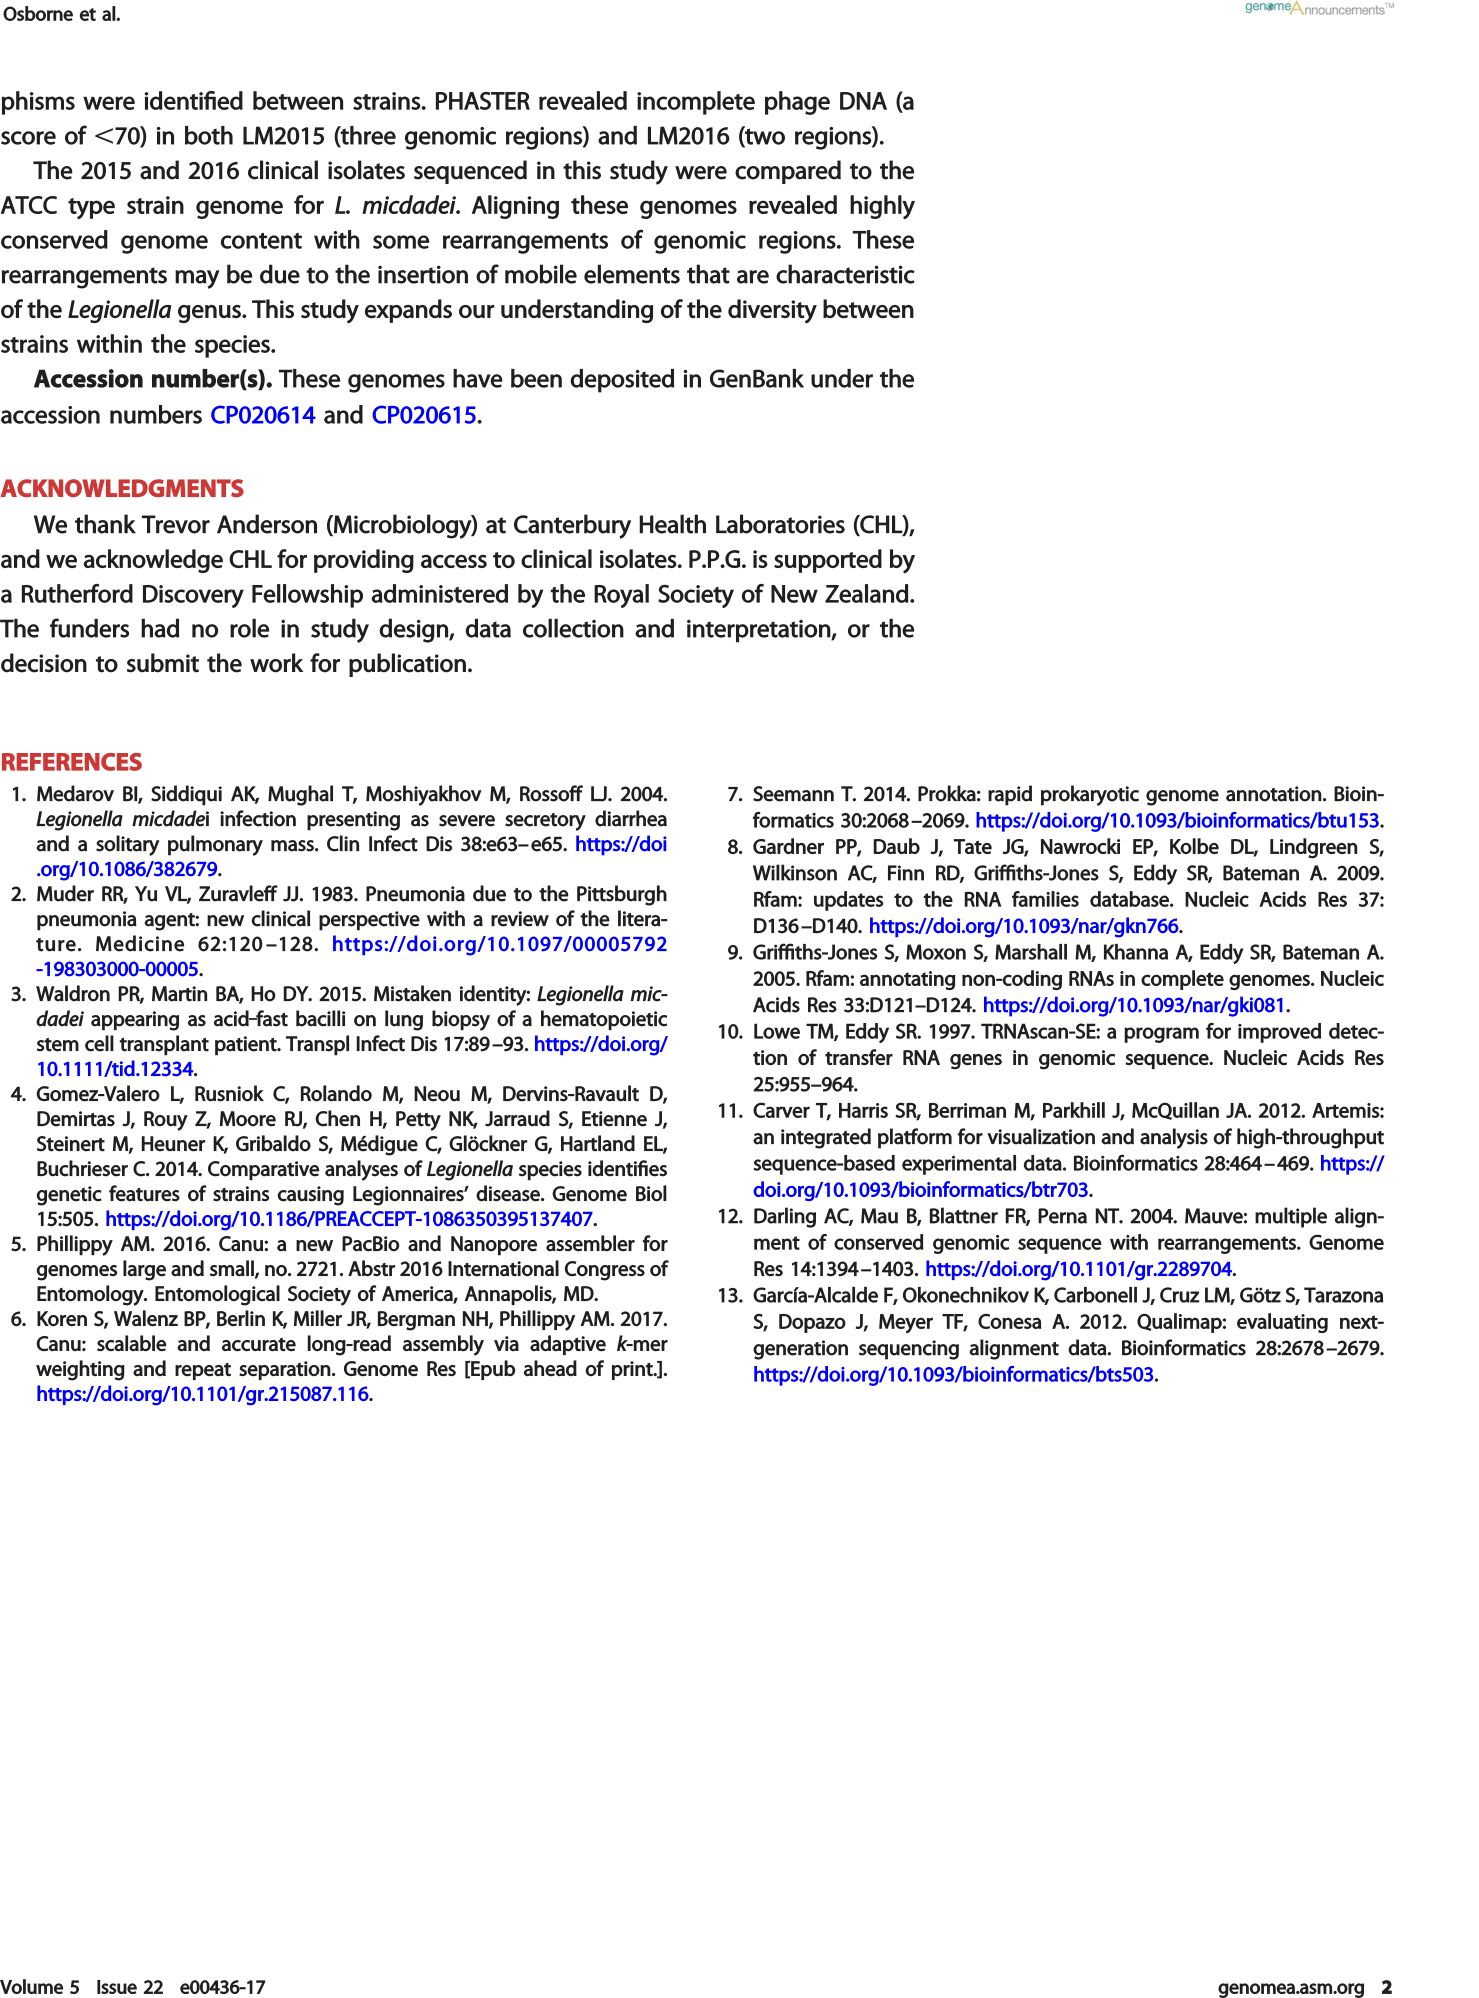
\includegraphics[width=\linewidth]{other/legionella_2.png}
\end{figure}
\cleardoublepage

\footnotesize
\chapter{Chapter 3 Appendices}
\begin{table}[H]
    \footnotesize
    \centering
    \begin{tabular}{cccc}\toprule
    Dataset & E-value threshold & Number of results & Post-filtering \\\midrule
ST7/74 sRNAs & 0.01 & 108543 & 32575 \\
& 0.001 & 86942 & 32511 \\
sRNA flanking regions & 0.01 & 97104 \\
& 0.001 & 97104  \\\bottomrule
    \end{tabular}
    \caption[Effects of different E-value thresholding and filtering on homology search results]{Effects of different E-value thresholding and filtering on homology search results.}
    \label{tab:e_value_tests}
\end{table}
\begin{footnotesize}
\begin{longtable}{ll}
    \toprule
sRNA & Other names \\\midrule
    \endfirsthead
\textit{STnc1010} & \textit{STnc900} \\
\textit{DapZ} & \textit{STnc1020, STnc820} \\
\textit{STnc470}& \textit{STnc910} \\
\textit{SroA}& \textit{tpe79} \\
\textit{SgrS}& \textit{ryaA} \\
\textit{SraA}& \textit{psrA/t15} \\
\textit{ChiX}& \textit{MicM, SroB, RybC} \\
\textit{STnc480} & \textit{STnc970} \\
\textit{RybD} & \textit{STnc830} \\
\textit{RybB}& \textit{p25} \\
\textit{IsrB-1}& \textit{IS092} \\
\textit{SraB}& \textit{pke2} \\
\textit{IsrC}& \textit{IS102} \\
\textit{RyhB-2}& \textit{isrE, RfrB} \\
\textit{STnc540}& \textit{sRNA14} \\
\textit{RprA}& \textit{IS083} \\
\textit{RydB}& \textit{tpe7, IS082} \\
\textit{MgrR}& \textit{STnc560} \\
\textit{RyjB}& \textit{STnc1120} \\
\textit{RydC}& \textit{IS067} \\
\textit{MicC}& \textit{IS063, tke8} \\
\textit{FnrS}& \textit{STnc580} \\
\textit{SraC}& \textit{RyeA} \\
\textit{SdsR}& \textit{RyeB, tpke79} \\
\textit{STnc1690}& \textit{STnc1690} \\
\textit{STnc200}& \textit{STnc200} \\
\textit{RyeF}& \textit{STnc860} \\
\textit{RyeC}& \textit{tp11, SibA} \\
\textit{STnc1150}& \textit{STnc2060} \\
\textit{CyaR}& \textit{ryeE} \\
\textit{STnc2070}& \textit{STnc1370} \\
\textit{RyfA}& \textit{tp1, PAIR3} \\
\textit{GlmY}& \textit{tke1, sroF} \\
\textit{MicA}& \textit{sraD} \\
\textit{InvR}& \textit{STnc270} \\
\textit{GcvB}& \textit{IS145} \\
\textit{OmrA}& \textit{rygB} \\ 
\textit{OmrB}& \textit{t59, rygA, sraE} \\
\textit{SsrS}& \textit{6S} \\
\textit{RygC}& \textit{t27, SibC, QUAD1c} \\
\textit{STnc750}& \textit{sRNA8} \\
\textit{RygD}& \textit{tp8, SibD, C0730} \\
\textit{SraF} & \textit{tpk1, IS160, PRE-element} \\
\textit{ArcZ}& \textit{SraH, ryhA} \\
\textit{RyhB-1}& \textit{SraI, IS176, RfrA} \\
\textit{STnc770}& \textit{sRNA6} \\
\textit{STnc1430}& \textit{STM3624.1N} \\
\textit{GlmZ}& \textit{k19, ryiA, SraJ} \\
\textit{Spf}& \textit{Spot 42} \\
\textit{CsrC}& \textit{SraK, RyiB, tpk2} \\
\textit{STnc810}& \textit{STnc2120} \\
\textit{SraL}& \textit{ryjA} \\
\textit{STnc630}& \textit{STnc2140} \\
\bottomrule
    \caption[Alternative sRNA gene names]{Alternative sRNA gene names}
    \label{tab:sRNA_alternative_names}
\end{longtable}
\end{footnotesize}
\begin{footnotesize}
\begin{longtable}{p{7cm}p{7cm}}
    \toprule
EggNOG MGE protein descriptions &\\\midrule
    \endfirsthead
CcdB-like toxin protein & cell killing protein encoded within\\ cryptic prophage & Transposase \\
PipA protein &  anti-termination protein \\
transposase & Integrase \\
Inherit from COG: Antirepressor & Inherit from COG: transposase\\
Integrase catalytic subunit & IS630 family transposase \\
Major tail protein & Phage transcriptional regulator, AlpA \\
Plasmid maintenance system antidote protein & plasmid maintenance system antidote protein, xre family \\
Protein of unknown function (DUF1019) & Transposase IS116 IS110 IS902 \\
Transposase is3 is911 & replication protein O \\
small terminase subunit & Tail assembly protein \\
tail length tape measure & Terminase, large subunit \\
bacteriophage protein & enhancing factor (Viral) \\
Antitermination protein & Minor Tail Protein \\
P2 GpU Family Protein & phage baseplate \\
phage minor tail protein L & phage protein \\
Prophage membrane protein & Qin prophage\\
CcdA protein & Excisionase \\
tail component of prophage & tail component of prophage CP-933K\\
Tail Fiber Assembly protein & tail fiber protein \\
Toxic component of a toxin-antitoxin (TA) module. A & NinB protein\\
late control & Late control D family protein\\
excisionase & Tail fiber protein \\
transcriptional activator, Ogr delta & lambda NinG\\
phage regulatory protein, rha family & Pfam:DUF1813 \\
DNA-binding prophage protein & Pfam:Transposase\\
phage holin & is1 orf2\\
this blockage is overcome by subsequent expression of antitoxin HigA. Overexpression causes cleavage of a number of mRNAs in a translation-dependent fashion, suggesting this is an mRNA interferase\\
\bottomrule
    \caption[Manually curated EggNOG MGE protein descriptions]{Manually curated EggNOG MGE protein descriptions.}
    \label{tab:manual_MGE_terms}
\end{longtable}
\end{footnotesize}



